\chapter{Các tật của mắt và cách khắc phục}
\section{Lý thuyết trọng tâm}

\subsection{Mắt cận và cách khắc phục}
Mắt cận là mắt khi không điều tiết, có tiêu điểm nằm trước võng mạc.
\begin{center}
	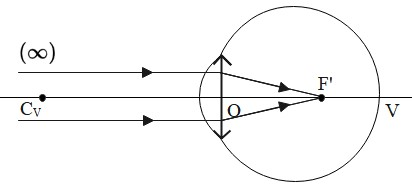
\includegraphics[scale=0.8]{../figs/VN11-PH-40-L-028-3-h37.jpg}
\end{center}

Đặc điểm:
\begin{itemize}
	\item Khi không điều tiết: $f_\text{max}< \text{OV}$.
	\item Không thể nhìn được rõ các vật ở xa vô cực.
	\item Điểm cực cận và điểm cực viễn dời rất gần mắt.
\end{itemize}

Sửa tật cận thị là làm cho mắt cận thị có thể nhìn rõ các vật ở vô cực mà không phải điều tiết. Cách sửa: đeo \textit{thấu kính phân kỳ} thích hợp sao cho nhìn rõ vật ở vô cực mà không phải điều tiết. Suy ra ảnh sẽ nằm tại tiêu diện của kính hay trùng với điểm cực viễn $\text{C}_\text{v}$.
\begin{center}
	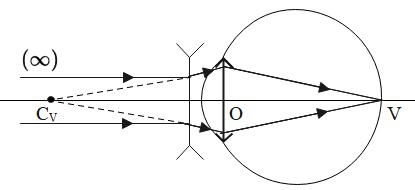
\includegraphics[scale=0.8]{../figs/VN11-PH-40-L-028-3-h38.jpg}
\end{center}

Công thức xác định vị trí ảnh: $$\dfrac{1}{f}=\dfrac{1}{d}+\dfrac{1}{d'}.$$

Ta có: $d=\infty, \ d'=-\text{OV}$ nên:
\begin{equation}
 D=\dfrac{1}{f}=-\dfrac{1}{\text{OV}}
\end{equation}


\subsection{Mắt viễn và cách khắc phục}
Mắt viễn là mắt khi không điều tiết, có tiêu điểm nằm sau võng mạc.
	\begin{center}
		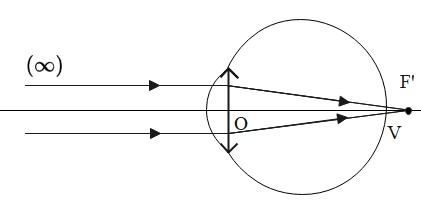
\includegraphics[scale=0.8]{../figs/VN11-PH-40-L-028-3-h39.jpg}
	\end{center}

 Đặc điểm:
	\begin{itemize}
		\item Khi không điều tiết: $f_\text{max}> \text{OV}$.
		\item Khi nhìn các vật ở xa vô cực, mắt phải điều tiết.
		\item Điểm cực cận và điểm cực viễn dời xa mắt.
	\end{itemize}
	
Sửa tật viễn thị là làm cho mắt viễn thị có thể nhìn rõ các vật ở gần như mắt không tật (có điểm $\text{C}_\text{c}$ cách mắt 25 cm). Cách sửa: đeo thấu kính hội tụ thích hợp sao cho nhìn rõ vật ở gần như mắt bình thường. 
	\begin{center}
		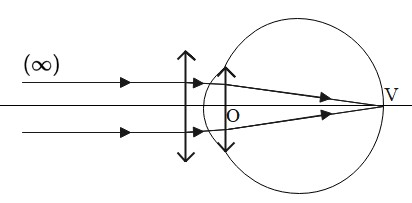
\includegraphics[scale=0.8]{../figs/VN11-PH-40-L-028-3-h40.jpg}
	\end{center}


\subsection{Mắt lão và cách khắc phục}
 Mắt lão là mắt khi lớn tuổi có điểm cực cận lùi ra xa mắt do khả năng điều tiết giảm.

Đặc điểm:
	\begin{itemize}
		\item Mắt lão vẫn nhìn được các vật ở vô cực mà không phải điều tiết (giống mắt không tật).
		\item Điểm cực cận dời xa mắt (giống mắt viễn thị).
	\end{itemize}

 Sửa tật lão thị là làm cho mắt lão thị có thể nhìn rõ các vật ở gần như mắt không tật (có điểm $\text{C}_\text{c}$ cách mắt 25 cm). Cách sửa: Đeo thấu kính hội tụ thích hợp tương tự như người bị viễn thị. 

Đặc biệt, người có mắt cận khi lớn tuổi thường phải đeo kính phân kỳ để nhìn xa và đeo kính hội tụ để nhìn gần. 
Người ta thường thực hiện loại "kính hai tròng" có phần trên phần kỳ và phần dưới hội tụ. 

	\luuy{
	\begin{itemize}
		\item Có thể đưa bài toán sửa tật của mắt về dạng bài toán hệ thấu kính ghép trong đó có một thấu kính là thủy tinh thể.
		\item Với mỗi mắt, khoảng cách OV không thay đổi (có giá trị từ $\text{1,5}\ \text{cm}$ đến $\text{2,2}\ \text{cm}$). Ảnh sau cùng của vật tạo bởi hệ ghép tại điểm vàng V trên võng mạc.
			\end{itemize}
	
}

\section{Bài tập }
\begin{dang}{Mắt cận thị và cách sửa tật cận thị}
\end{dang}
\textbf{Phương pháp giải}

Đeo thấu kính phân kỳ để nhìn xa như người bình thường, tức là vật ở vô cực cho ảnh ảo qua kính nằm ở điểm cực viễn.

Sơ đồ tạo ảnh:
$${\text{S}\ (d=\infty)}\xrightarrow[]{\text{O}_\text{k}} \text{S}'\equiv \text{C}_\text{v}  \xrightarrow[]{\text{O}}\text{S}''\equiv \text{V}.$$

\begin{center}
	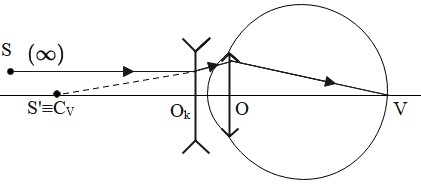
\includegraphics[scale=0.8]{../figs/VN11-PH-40-L-028-3-h41.jpg}
\end{center}

Khi đeo kính cách mắt một đoạn $l$: 
	$$d=\infty\Rightarrow d'=-\text{O}_\text{k}\text{C}_\text{v}=-(\text{O}\text{C}_\text{v}-l)=f_\text{k},$$ 
với $l=\text{O}\text{O}_\text{k}$ là khoảng cách từ kính đến mắt.

Khi đeo kính sát mắt $(\text{O}_\text{k}\equiv \text{O})$: $l=0\Rightarrow d'=-\text{OC}_\text{v}=f_\text{k}$. 

\vspace{1em}
\viduii{3}{
Một người cận thị có khoảng nhìn rõ từ $\text{12,5}\ \text{cm}$ đến $\text{50}\ \text{cm}$. Khi đeo kính chữa tật của mắt, người này nhìn rõ được các vật đặt gần nhất cách mắt
\begin{mcq}(4)
	\item $\text{11,7}\ \text{cm}$
	\item $\text{16,7}\ \text{cm}$
	\item $\text{17,5}\ \text{cm}$
	\item $\text{22,5}\ \text{cm}$
\end{mcq}}{
\begin{center}
	\textbf{Hướng dẫn giải:}
\end{center}

{ Tiêu cự của thấu kính đeo là $f=-\text{OC}_\text{v}=-50\ \text{cm}$.
	
	Khi đeo kính, vật nằm tại một điểm xác định qua kính cho ảnh ảo nằm tại $\text{C}_\text{c}$.
	
Công thức thấu kính: $\dfrac{1}{f}=\dfrac{1}{d}+\dfrac{1}{d'}$, với $f=-50\ \text{cm}, \ d=-\text{12,5}\ \text{cm}$.

Suy ra $d=\text{16,7}\ \text{cm}$.

Khi đeo kính chữa tật của mắt, người này nhìn rõ được các vật đặt gần nhất cách mắt $\text{16,7}\ \text{cm}$.

\textbf{	Đáp án: B.}
	
}}

\viduii{3}{

Một người đeo một kính có $D_1 = 1\ \text{dp}$  thì có thể nhìn rõ những vật ở cách mắt từ $\dfrac{100}{7}$ cm đến 25 cm. Mắt bị tật gì? Để sửa tật cần đeo kính có độ tụ $D_2$ bằng bao nhiêu? Biết kính đeo sát mắt.
\begin{mcq}
	\item Mắt bị tật cận thị, $D_2 =-3\ \text{dp}$. 
	\item Mắt bị tật viễn thị, $D_2 =3\ \text{dp}$. 
	\item Mắt bị tật cận thị, $D_2 =-2\ \text{dp}$. 
	\item Mắt bị tật viễn thị, $D_2 =2\ \text{dp}$. 
\end{mcq}}{
\begin{center}
	\textbf{Hướng dẫn giải:}
\end{center}

{ Kính đeo sát mắt: $l = 0$.
	
 Tiêu cự kính đeo: $f_\text{k}=\dfrac{1}{D}=1\ \text{m}=100\ \text{cm}$.
 
Khi đeo kính: Vật xa nhất mắt nhìn rõ là vật qua kính cho ảnh ở cực viễn của mắt. 

Ta có:   $d_\text{v}=25\ \text{cm},\ f_\text{k}=100\ \text{cm},  \ d'_\text{v}=-\text{OC}_\text{v}=?$

	Từ $\dfrac{1}{f_\text{k}}=\dfrac{1}{d_\text{v}}+\dfrac{1}{d'_\text{v}}\Rightarrow d'_\text{v}=-\text{33,33}\ \text{cm}\Rightarrow \text{OC}_\text{v}= \text{33,33}\ \text{cm}$.
	
	Vật gần nhất qua thấu kính cho ảnh ảo ở cực cận của mắt.
	
	Ta có:   $d_\text{c}=\dfrac{100}{7}\ \text{cm},\ f_\text{k}=100\ \text{cm},  \ d'_\text{c}=-\text{OC}_\text{c}=?$
	
	Từ $\dfrac{1}{f_\text{k}}=\dfrac{1}{d_\text{c}}+\dfrac{1}{d'_\text{c}}\Rightarrow d'_\text{c}=-\text{16,67}\ \text{cm}\Rightarrow \text{OC}_\text{c}= \text{16,67}\ \text{cm}$.
	
	Vậy khi chưa đeo kính người này nhìn được vật cách mắt từ $\text{16,67}\ \text{cm}$  đến $\text{33,33}\ \text{cm}$. 
	
	Suy ra người này bị cận thị (do chỉ nhìn xa tối đa $\text{33,33}\ \text{cm}$).
	
	Muốn sửa tật cận thị (hay muốn nhìn vật ở xa vô cực mà không cần điều tiết) cần đeo kính phân kỳ có tiêu cự sao cho vật ở xa qua kính cho ảnh ảo ở cực viễn của mắt.
	
	Do kính đeo sát mắt: $f_2 = -\text{OC}_\text{v} = -\text{33,33}\ \text{cm} $.
	
	Độ tụ của kính: $D_2=\dfrac{1}{f_2}=-3\ \text{dp}$.
		

\textbf{	Đáp án: A.}
	
}}


\begin{dang}{Mắt viễn thị và cách sửa tật viễn thị}
\end{dang}
\textbf{Phương pháp giải}

\textbf{Trường hợp 1: nhìn vật ở gần nhất như mắt bình thường} cần đeo kính hội tụ có tiêu cự sao cho vật này qua kính cho ảnh ảo ở cực cận của mắt.

Liên hệ giữa tiêu cự thấu kính $f_\text{k}$, khoảng cách từ vật đến kính $d_\text{C}$ và khoảng cách từ ảnh đến kính $d'_\text{C}=-(\text{O}\text{C}_\text{c}-l)$:
$$\dfrac{1}{f_\text{k}}=\dfrac{1}{d_\text{C}}+\dfrac{1}{d'_\text{C}}$$

Ta cần xác định rõ các dữ liệu đề cho để suy ra đại lượng cần tìm.

\luuy{
	Ảnh ảo lúc này là vật thật đối với thủy tinh thể, qua thủy tinh thể cho ảnh thật trên võng mạc. Mắt nhìn rõ vật này khi đã điều tiết tối đa.
	
}

\textbf{Trường hợp 2: muốn nhìn vật ở xa vô cực mà không cần điều tiết} cần đeo kính hội tụ có tiêu cự sao cho vật ở vô cực qua kính cho ảnh thật ở cực viễn của mắt 

Liên hệ giữa tiêu cự thấu kính $f_\text{k}$, khoảng cách từ vật đến kính $d_\text{V}=\infty$ và khoảng cách từ ảnh đến kính $d'_\text{C}=\text{O}\text{C}_\text{v}+l$:
$$\dfrac{1}{f_\text{k}}=\dfrac{1}{d_\text{V}}+\dfrac{1}{d'_\text{V}}.$$

Ta cần xác định rõ các dữ liệu đề cho để suy ra đại lượng cần tìm.

\luuy{
	Ảnh ảo lúc này là vật thật đối với thủy tinh thể, qua thủy tinh thể cho ảnh thật trên võng mạc. Mắt nhìn rõ vật này khi đã điều tiết tối đa.
	Khi điểm cực viễn là điểm ảo (ở sau mắt viễn thị) nên ảnh tại cực viễn là ảnh thật, ta có: $d'_\text{C}=\text{O}\text{C}_\text{v}+l$.
	
}

\luuy{
\textbf{Khi chưa đeo kính:} Đề cho khoảng nhìn rõ tức là cho $\text{OC}_\text{c},\text{OC}_\text{v}$. 
Ngược lại khi đề yêu cầu tìm khoảng nhìn rõ khi chưa đeo kính thì ta cần tìm $\text{OC}_\text{c}, \ \text{OC}_\text{v}$, nghĩa là tìm được $d'_\text{C}, \  d'_\text{v} $.

\textbf{Khi đeo kính:} Đề cho khoảng nhìn rõ tức là cho $d_\text{C}, \ d_\text{v}$. Ngược lại khi đề yêu cầu tìm khoảng nhìn rõ khi đeo kính thì ta cần tìm được $d_\text{C}, \ d_\text{v}$.

	
}



\viduii{2}{

Một người viễn thị có điểm cực cận cách mắt 60 cm. Khi đeo kính có độ tụ 1 dp, kính đeo sát mắt, người này sẽ nhìn rõ được những vật gần nhất cách mắt
\begin{mcq}(4)
	\item $\text{150}\ \text{cm}$.
	\item $\text{37,5}\ \text{cm}$.
	\item $\text{40}\ \text{cm}$.
	\item $\text{26,7}\ \text{cm}$.
\end{mcq}}{
\begin{center}
	\textbf{Hướng dẫn giải:}
\end{center}

{ $f_\text{k}=\dfrac{1}{D}=1\ \text{m}= 100\ \text{cm}$.
	
$d_\text{C}$ là khoảng cách từ vật đến kính.
	
 $d'_\text{C}=-(\text{O}\text{C}_\text{c}-l)=\text{O}\text{C}_\text{c}=-60 \ \text{cm}$ (do $l=0$).
 
 $\dfrac{1}{f_\text{k}}=\dfrac{1}{d_\text{C}}+\dfrac{1}{d'_\text{C}}$
 
 $\Rightarrow d_\text{C}= \text{37,5}\ \text{cm}$.
 
\textbf{	Đáp án: B.}
}
}
\viduii{2}{
Mắt viễn nhìn rõ được vật đặt cách mắt gần nhất 50 cm. Để nhìn rõ vật đặt cách mắt gần nhất 25 cm cần đeo kính (kính cách mắt 1 cm) có độ tụ là
\begin{mcq}(4)
	\item $\text{2,13}\ \text{dp}$.
	\item $\text{3,13}\ \text{dp}$.
	\item $\text{4,13}\ \text{dp}$.
	\item $\text{5,13}\ \text{dp}$.
\end{mcq}}{
\begin{center}
	\textbf{Hướng dẫn giải:}
\end{center}

{ 	$d_\text{C}=24 \ \text{cm}$ là khoảng cách từ vật đến kính.
	
	$d'_\text{C}=-(\text{O}\text{C}_\text{c}-l)=-49\ \text{cm}$ (do $l=1\ \text{cm}$).
	
	$\dfrac{1}{f_\text{k}}=\dfrac{1}{d_\text{C}}+\dfrac{1}{d'_\text{C}}\Rightarrow f_\text{k}=\text{47,04}\ \text{cm}=\text{0,4704}\ \text{m}$.
	
	$D=\dfrac{1}{f_\text{k}}=\text{2,13}\ \text{dp}$.
	
\textbf{	Đáp án: A.}
}}


